\section{}
\label{sec:problem4}
%%%%%%%%%%%%%%%%%%%%%%%%%%%%%%%%%%%%%%%%%%%%%%%%%%%%%%%%%%%%%%%%%%%%%%

We use the biological cell data and want to model a repulsive event RF with a strauss model. This model is on conditional form given the event count $k_D = k$ we have the realizations given by Equation \ref{eq:straureal}. 
\begin{equation}
    \begin{array}{rcl}
        \left[\matr{X}_D^S \given k_D = k\right] & \sim & p(\vect{x}_1,\vect{x}_2,...,\vect{x}_k \given k_D = k) \\
         & = & \mathrm{const} \times \prod\limits_{i,j\in \{1,2,...k\}} exp\{-\phi(\vect{x}_i-\vect{x}_j)\}
    \end{array}
    \label{eq:straureal}
\end{equation}

Then let the distance be $\tau_{ij} = |\vect{\tau}_{ij}| \in \R_\oplus; \vect{\tau}_{ij} = \vect{x}_i - \vect{x}_j$, where $\phi(\tau)$ is given by equation 
\begin{equation}
    \phi(\tau) = \begin{cases}
                    \phi_0; & 0 \leq \tau \leq \tau_0\\
                    \phi_0 exp\{-\phi_1[\tau-\tau_0]\}; & \tau > \tau_0
                \end{cases},
    \label{eq:interfunction}
\end{equation}
where $\tau_0 \in R_\oplus$ and $\phi_0,\phi_1 \in R_+$. This gives the model parameters for the Strauss-model $\vect{\theta} _{pS\given k} = [\tau_0,\phi_0,\phi_1]$.

\begin{figure}
    \centering
    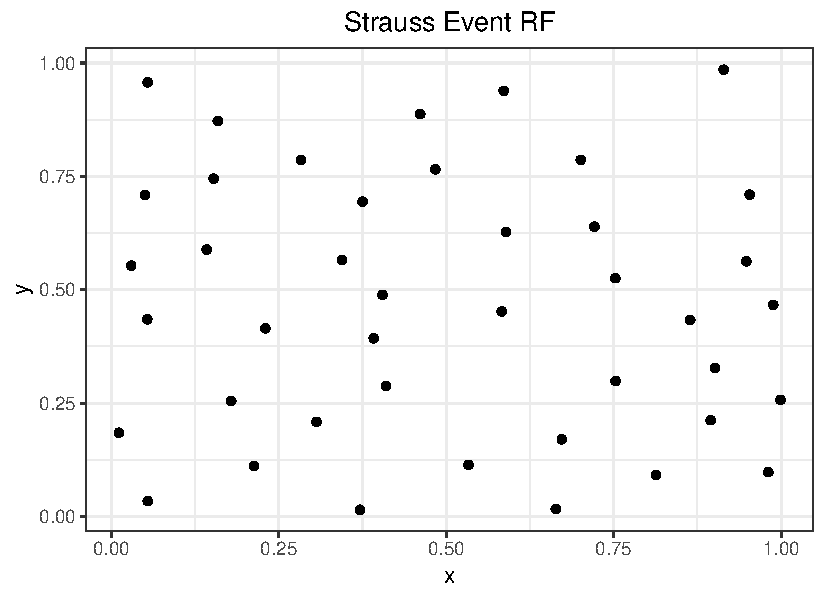
\includegraphics[scale=0.95]{figures/repulsive_event_rf.pdf}
    \caption{}
    \label{fig:repulsive_event_rf}
\end{figure}

\begin{figure}
    \centering
    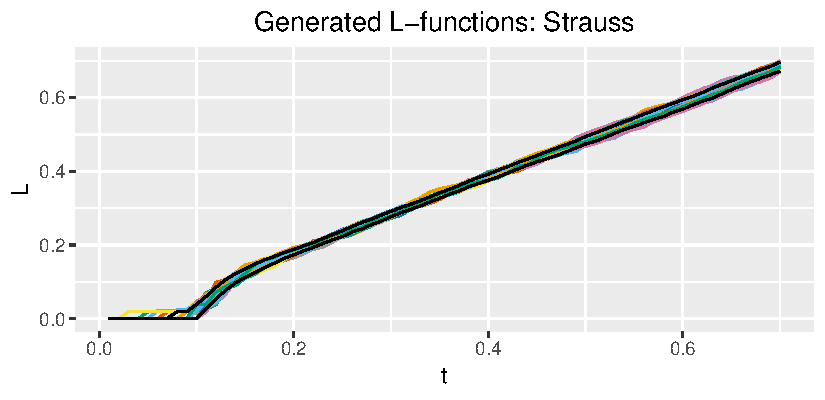
\includegraphics[scale=0.65]{figures/gen_strauss_l.pdf}
    \caption{}
    \label{fig:gen_strauss_l}
\end{figure}

\begin{figure}
    \centering
    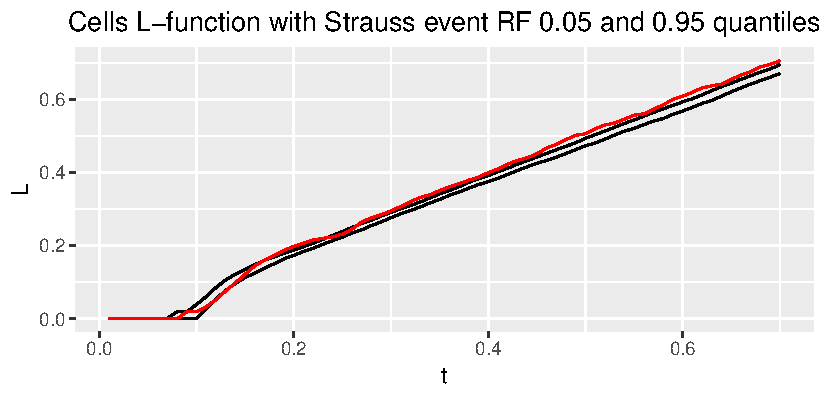
\includegraphics[scale=0.65]{figures/strauss_quant1.pdf}
    \caption{}
    \label{fig:strauss_quant1}
\end{figure}

\begin{figure}
    \centering
    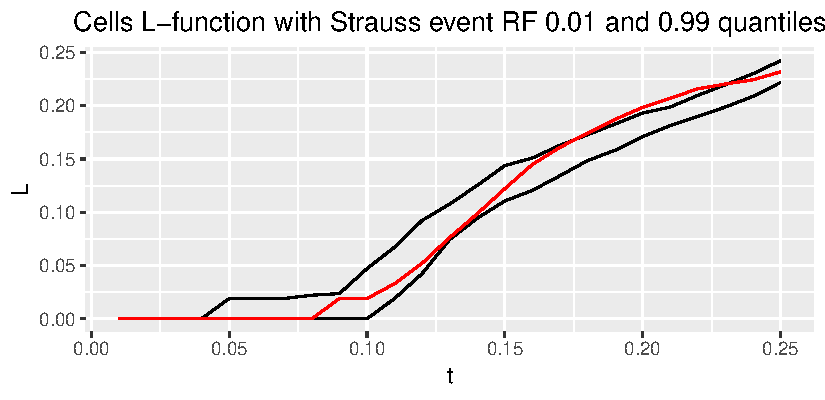
\includegraphics[scale=0.65]{figures/strauss_quant2.pdf}
    \caption{}
    \label{fig:strauss  _quant2}
\end{figure}